\documentclass{standalone}
\usepackage{tikz}
\usetikzlibrary{calc}
\begin{document}

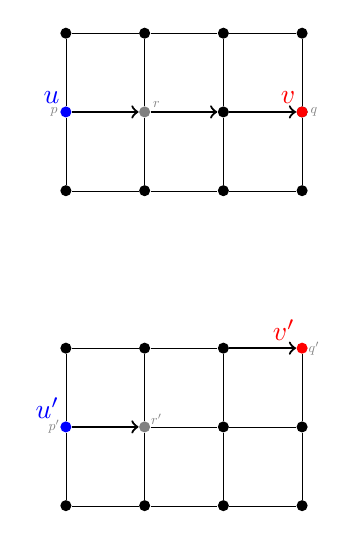
\begin{tikzpicture}[
  every node/.style={circle, fill=black, inner sep=1pt, minimum size=4pt}
]

  \node (a) at (0,6) {};
  \node (b) at (1,6){};
  \node (c) at (2,6){};
  \node (d) at (3,6){};
  \node[label={[blue]above left:$u$}] (e) at (0,5) [circle, color=blue] {};
  \node[draw=none, fill=none, scale=0.5, text=gray] (label2) at (-0.15,5) {$p$};
  \node (f) at (1,5) [color=gray]{};
  \node[draw=none, fill=none, scale=0.5, text=gray] (label3) at (1.15,5.1) {$r$};
  \node (g) at (2,5){};
  \node (h) at (3,5){};
  \node[label={[red]above left:$v$}] (h) at (3,5) [circle, color=red] {};
  \node[draw=none, fill=none, scale=0.5, text=gray] (label1) at (3.15,5) {$q$};
  \node (i) at (0,4){};
  \node (j) at (1,4){};
  \node (k) at (2,4){};
  \node (l) at (3,4){};

  \draw (a) edge[-, ultra thin] (b);
  \draw (a) edge[-, ultra thin] (e);
  \draw (b) edge[-, ultra thin] (c);
  \draw (b) edge[-, ultra thin] (f);
  \draw (c) edge[-, ultra thin] (d);
  \draw (c) edge[-, ultra thin] (g);
  \draw (d) edge[-, ultra thin] (h);
  \draw (e) edge[-, ultra thin] (i);
  \draw (i) edge[-, ultra thin] (j);
  \draw (f) edge[-, ultra thin] (j);
  \draw (j) edge[-, ultra thin] (k);
  \draw (g) edge[-, ultra thin] (k);
  \draw (k) edge[-, ultra thin] (l);
  \draw (h) edge[-, ultra thin] (l);
  \draw (e) edge[->, thick] (f);
  \draw (f) edge[->, thick] (g);
  \draw (g) edge[->, thick] (h);



  \node (a1) at (0,2){};
  \node (b1) at (1,2){};
  \node (c1) at (2,2){};
  \node[label={[red]above left:$v'$}] (d1) at (3,2) [circle, color=red] {};
  \node[draw=none, fill=none, scale=0.5, text=gray] (label1) at (3.15,2) {$q'$};
  \node[label={[blue]above left:$u'$}] (e1) at (0,1) [circle, color=blue] {};
  \node[draw=none, fill=none, scale=0.5, text=gray] (label2) at (-0.15,1) {$p'$};
  \node (f1) at (1,1) [color=gray]{};
  \node[draw=none, fill=none, scale=0.5, text=gray] (label3) at (1.15,1.1) {$r'$};
  \node (g1) at (2,1){};
  \node (h1) at (3,1){};
  \node (i1) at (0,0){};
  \node (j1) at (1,0){};
  \node (k1) at (2,0){};
  \node (l1) at (3,0){};


  \draw (a1) edge[-, ultra thin] (b1);
  \draw (a1) edge[-, ultra thin] (e1);
  \draw (b1) edge[-, ultra thin] (c1);
  \draw (b1) edge[-, ultra thin] (f1);
  \draw (c1) edge[->, thick] (d1);
  \draw (c1) edge[-, ultra thin] (g1);
  \draw (d1) edge[-, ultra thin] (h1);
  \draw (e1) edge[-, ultra thin] (i1);
  \draw (i1) edge[-, ultra thin] (j1);
  \draw (f1) edge[-, ultra thin] (j1);
  \draw (j1) edge[-, ultra thin] (k1);
  \draw (g1) edge[-, ultra thin] (k1);
  \draw (k1) edge[-, ultra thin] (l1);
  \draw (h1) edge[-, ultra thin] (l1);
  \draw (e1) edge[->, thick] (f1);
  \draw (f1) edge[-, ultra thin] (g1);
  \draw (g1) edge[-, ultra thin] (h1);

\end{tikzpicture}

\end{document}
